\documentclass[hyperref={pdfpagelabels=false}]{beamer}
\let\Tiny=\tiny
\mode<presentation>{
\usetheme{Singapore}
%\usecolortheme{lily}
\usefonttheme{serif}
}
\usepackage{default}
%\usepackage{ucs}
\usepackage[utf8]{inputenc}
\usepackage{gb4e}
\usepackage[T1]{fontenc}
\usepackage{ tipa }
\usepackage{qtree}
\usepackage{synttree}
\usepackage{color}
\usepackage{tree-dvips}
\usepackage[absolute,overlay]{textpos}
%\usepackage{covington-beamer}
\usepackage{lmodern}
\usepackage{hyperref}
\usepackage{natbib}
\usepackage{graphicx}
\usepackage{eso-pic}
\usepackage{booktabs}
\usepackage{tikz}
%\usepackage{memoir}
%\usepackage{relsize}
%\newcommand{\subscript}[1]{\raisebox{-0.25em}{\smaller #1}}
%\logo{\includegraphics[height=1cm]{nclcbelogomono.eps}}
\setbeamertemplate{footline}[frame number] 
%gets rid of navigation symbols
\setbeamertemplate{navigation symbols}{}

\title{How useful is information theory in predicting patterns of language use?}
\author{Joel C. Wallenberg\\\texttt{joel.wallenberg@ncl.ac.uk}}
\institute{
\includegraphics[scale = 0.2]{nclcbelogo.eps}}
%\date[]{\url{www.github.com/joelcw/constantentropy/ittalks/Wallenberg_cbe14May2019.pdf}}

\begin{document}

\begin{frame}[plain]
\titlepage
\end{frame}



\begin{frame}{Overall Points} 
\begin{itemize}
	\item \textbf{Shameless trick:} I don't really know *how* useful, and it's a limited domain of ``language use''.
	\begin{itemize}
	\item But the results are still very surprising, and at a level of detail that is only rivalled by one or two other results in the field.
	\end{itemize}
	\item \textbf{Main idea:} speakers unconsciously manipulate linguistic structure so that their utterances are more resistant to ``noise'' events that could destroy a whole message.
	\item ``noise'' is any interference, including: noise, memory, other processing costs, etc.
\end{itemize}
\end{frame}



\begin{frame}
\frametitle{Outline}
\tableofcontents
\end{frame}


\section{Information Theory}
\subsection{Crash Course}

\begin{frame}{Crash course} 
\begin{itemize}
	\item The amount of information a sender can theoretically communicate about an event is the uncertainty (``entropy'') the receiver has about the event.
	\item \citet{shannon1948}'s formula for information in an event with \textsl{n} discrete outcomes with probabilities p_1...p_n:
\end{itemize}
\begin{center}
	$$\sum_{1}^{n} p_i log_2 \frac{1}{p_i}$$
\end{center}
\begin{itemize}
	\item The $log_2 \frac{1}{p_i}$ part is the \textsl{information content} (or ``surprisal'') of an outcome.
\end{itemize}

\end{frame}

\begin{frame}{Crash course} 
\begin{itemize}
	\item The amount of information in a fair coin toss is 1 bit.
	\item The amount of information in an unfair coin toss with $$p = \frac{1}{3}, \frac{2}{3}$$ is less, even though less probable events have higher information content.
\end{itemize}
\begin{center}
	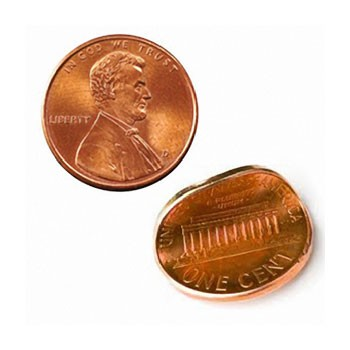
\includegraphics[scale=0.4]{bentcoin.jpg}
\end{center}
\end{frame}





\begin{frame}{``Uniform Information Density'' in language} 
\begin{center}
	Speakers spread information content across utterances as uniformly as possible, (possibly) so that utterances are more resistant to noise events \small{\citep{aylettturk2004,levyjaeger2007,levy2008a}}.
\end{center}
\begin{exe}
	\ex How big is the family $[$(that) you cook for$]$?
\end{exe}

\begin{center}
	If \textsl{that} is deleted, more information is carried by \textsl{you}, so information is more dense.
\end{center}


\end{frame}

\begin{frame}{``Uniform Information Density''} 
\begin{center}
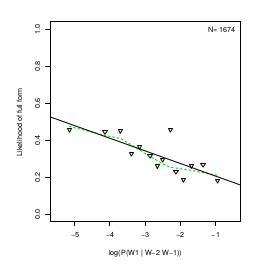
\includegraphics[scale=1.15]{levyPlot.png}
\end{center}

\end{frame}


\begin{frame}{UID and noise resistance} 

\begin{center}
\includegraphics[scale=0.585]{../sentence1info.png} 
\end{center}

\end{frame}

\begin{frame}{UID and noise resistance} 

\begin{center}
	\includegraphics[scale=0.585]{../sentence2info.png} 
\end{center}

\end{frame}


\subsection{Noise resistance simulation}

\begin{frame}{Noise resistance simulation} 
\begin{enumerate}
	\item Generate 10-item sequences of probabilities.
	\item Order them randomly, by size (``asymmetric''), or hyperdispersed (``optimised'').
	\item A noise event randomly destroys a 3-item sub-sequence.
	\item See how much information the noise events destroy (over many trials)!
\end{enumerate}
\end{frame}

\begin{frame}{Noise Resistance Simulation: proportion of bits lost} 

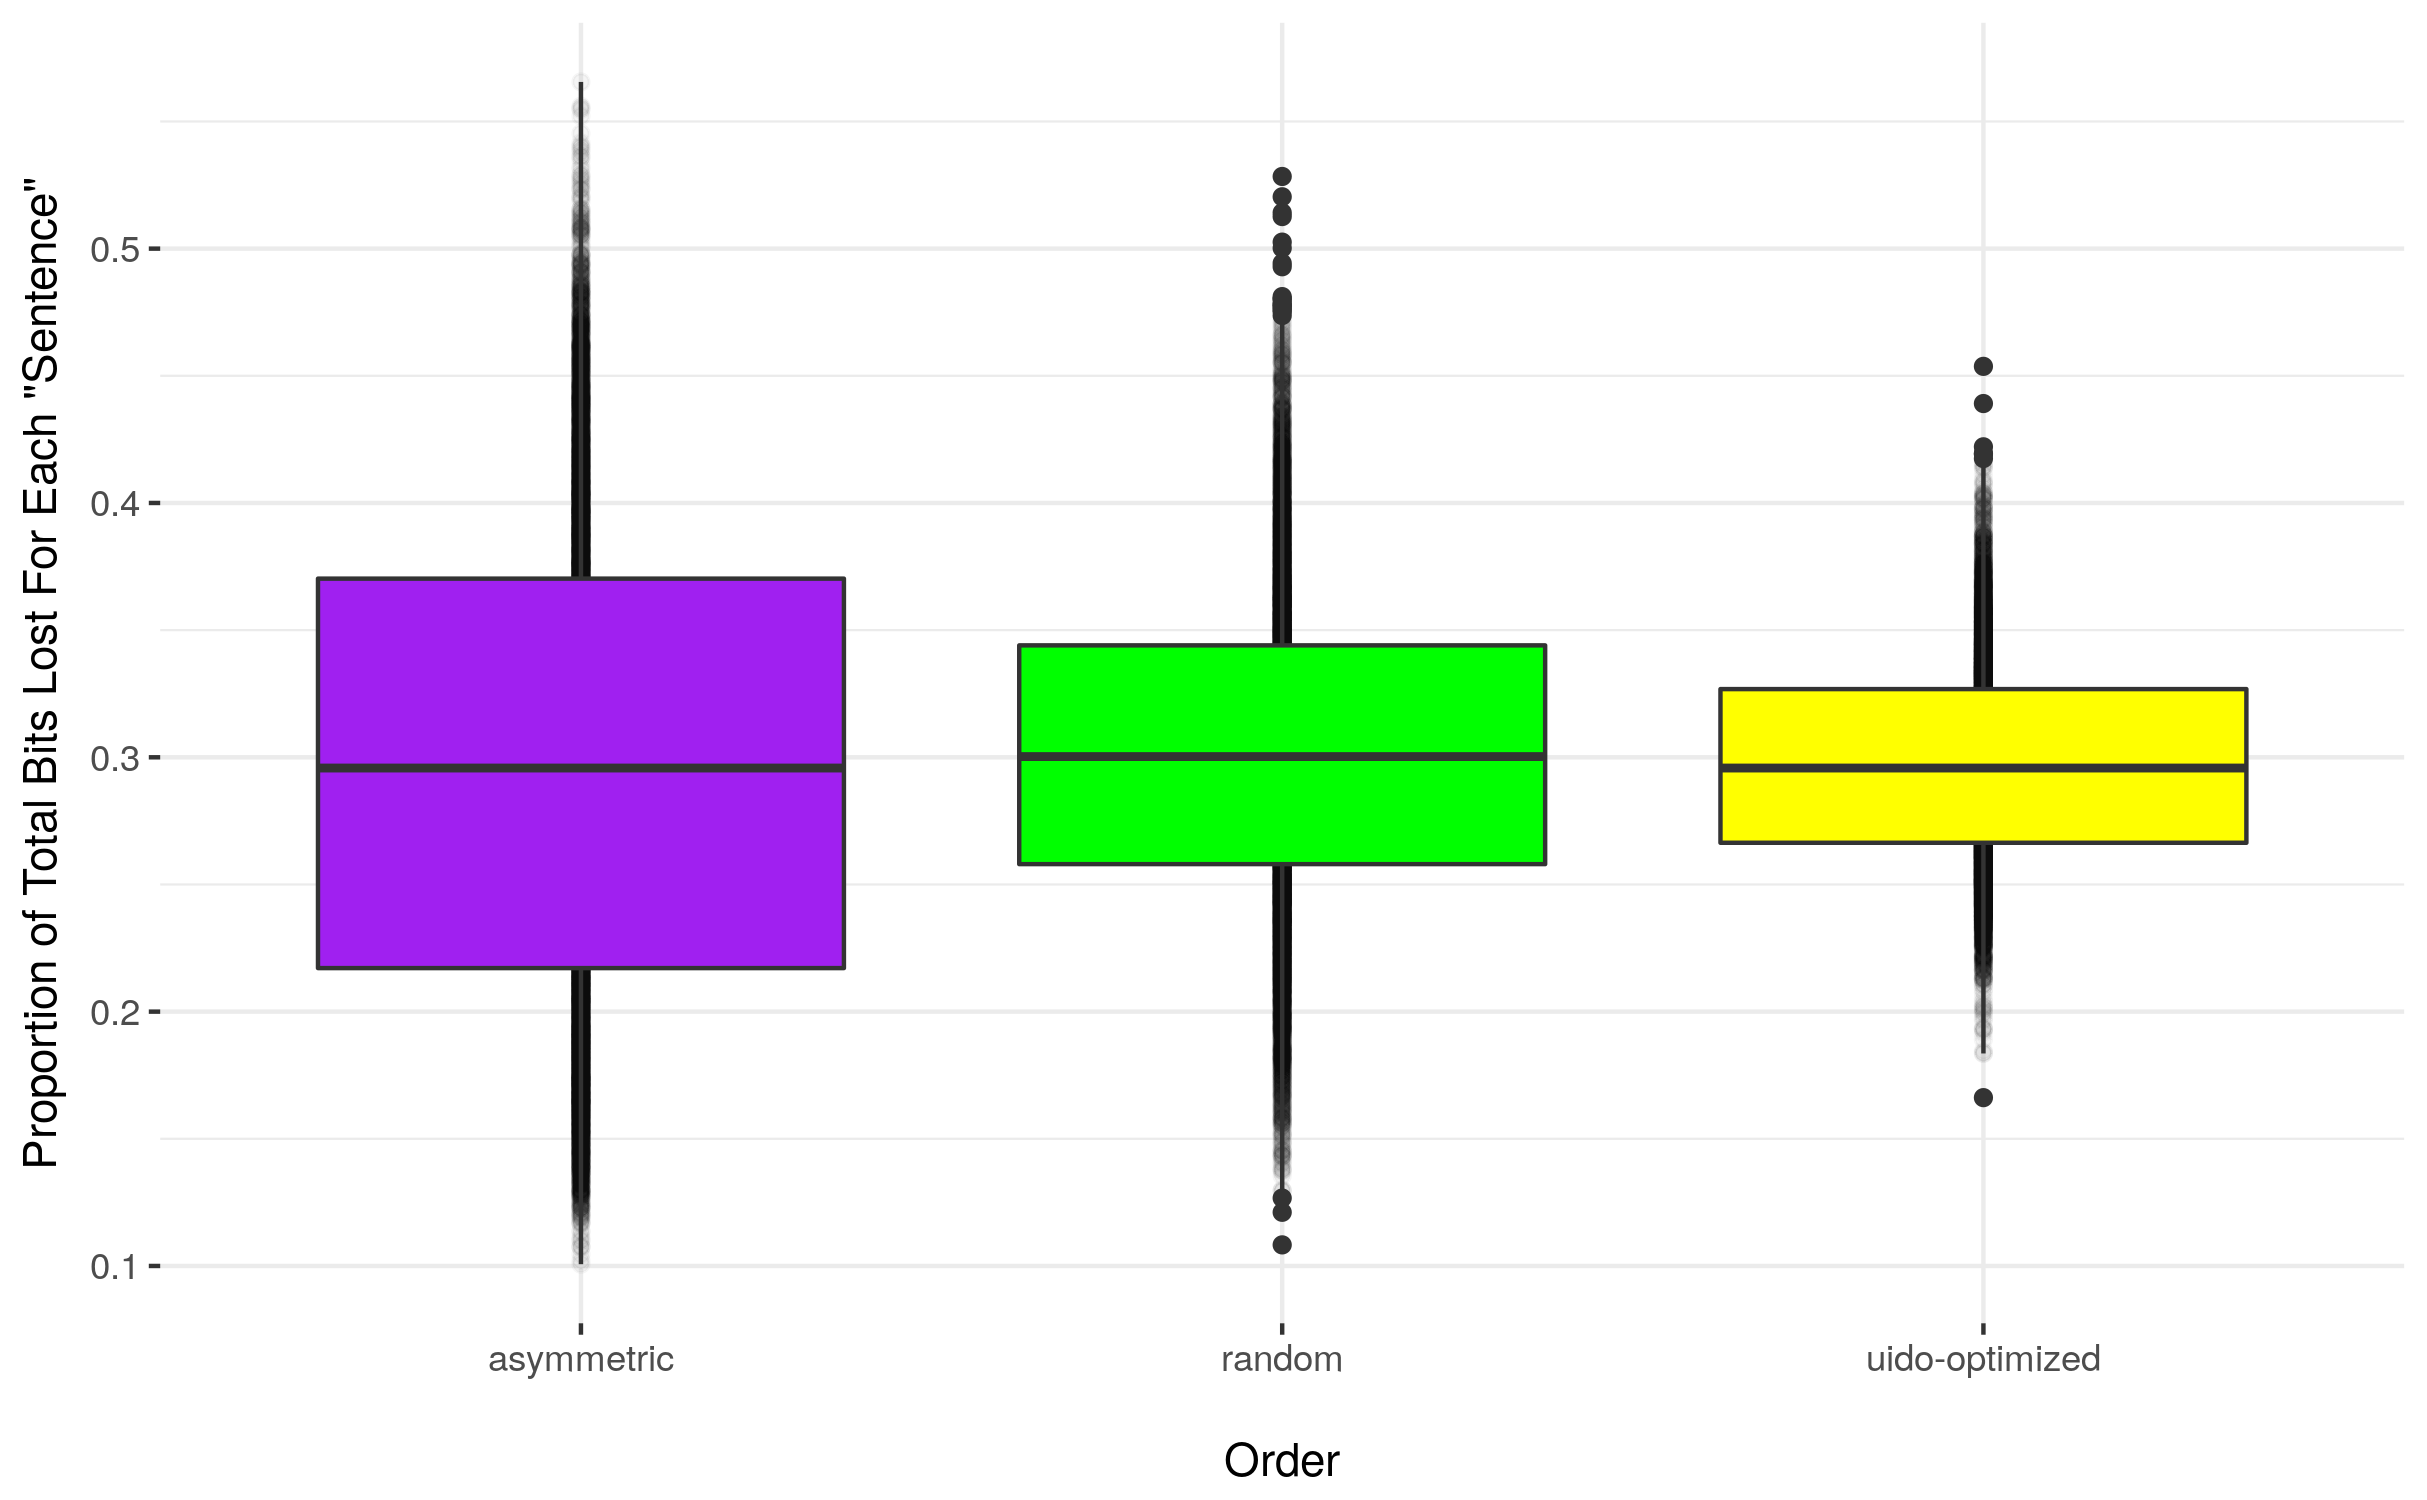
\includegraphics[width=1.15\textwidth]{../uid-sim-totalbits.png}


\end{frame}


\begin{frame}{Noise Resistance Sim: proportion of ``sentences'' where \\bits lost > 50\% bits in sentence} 



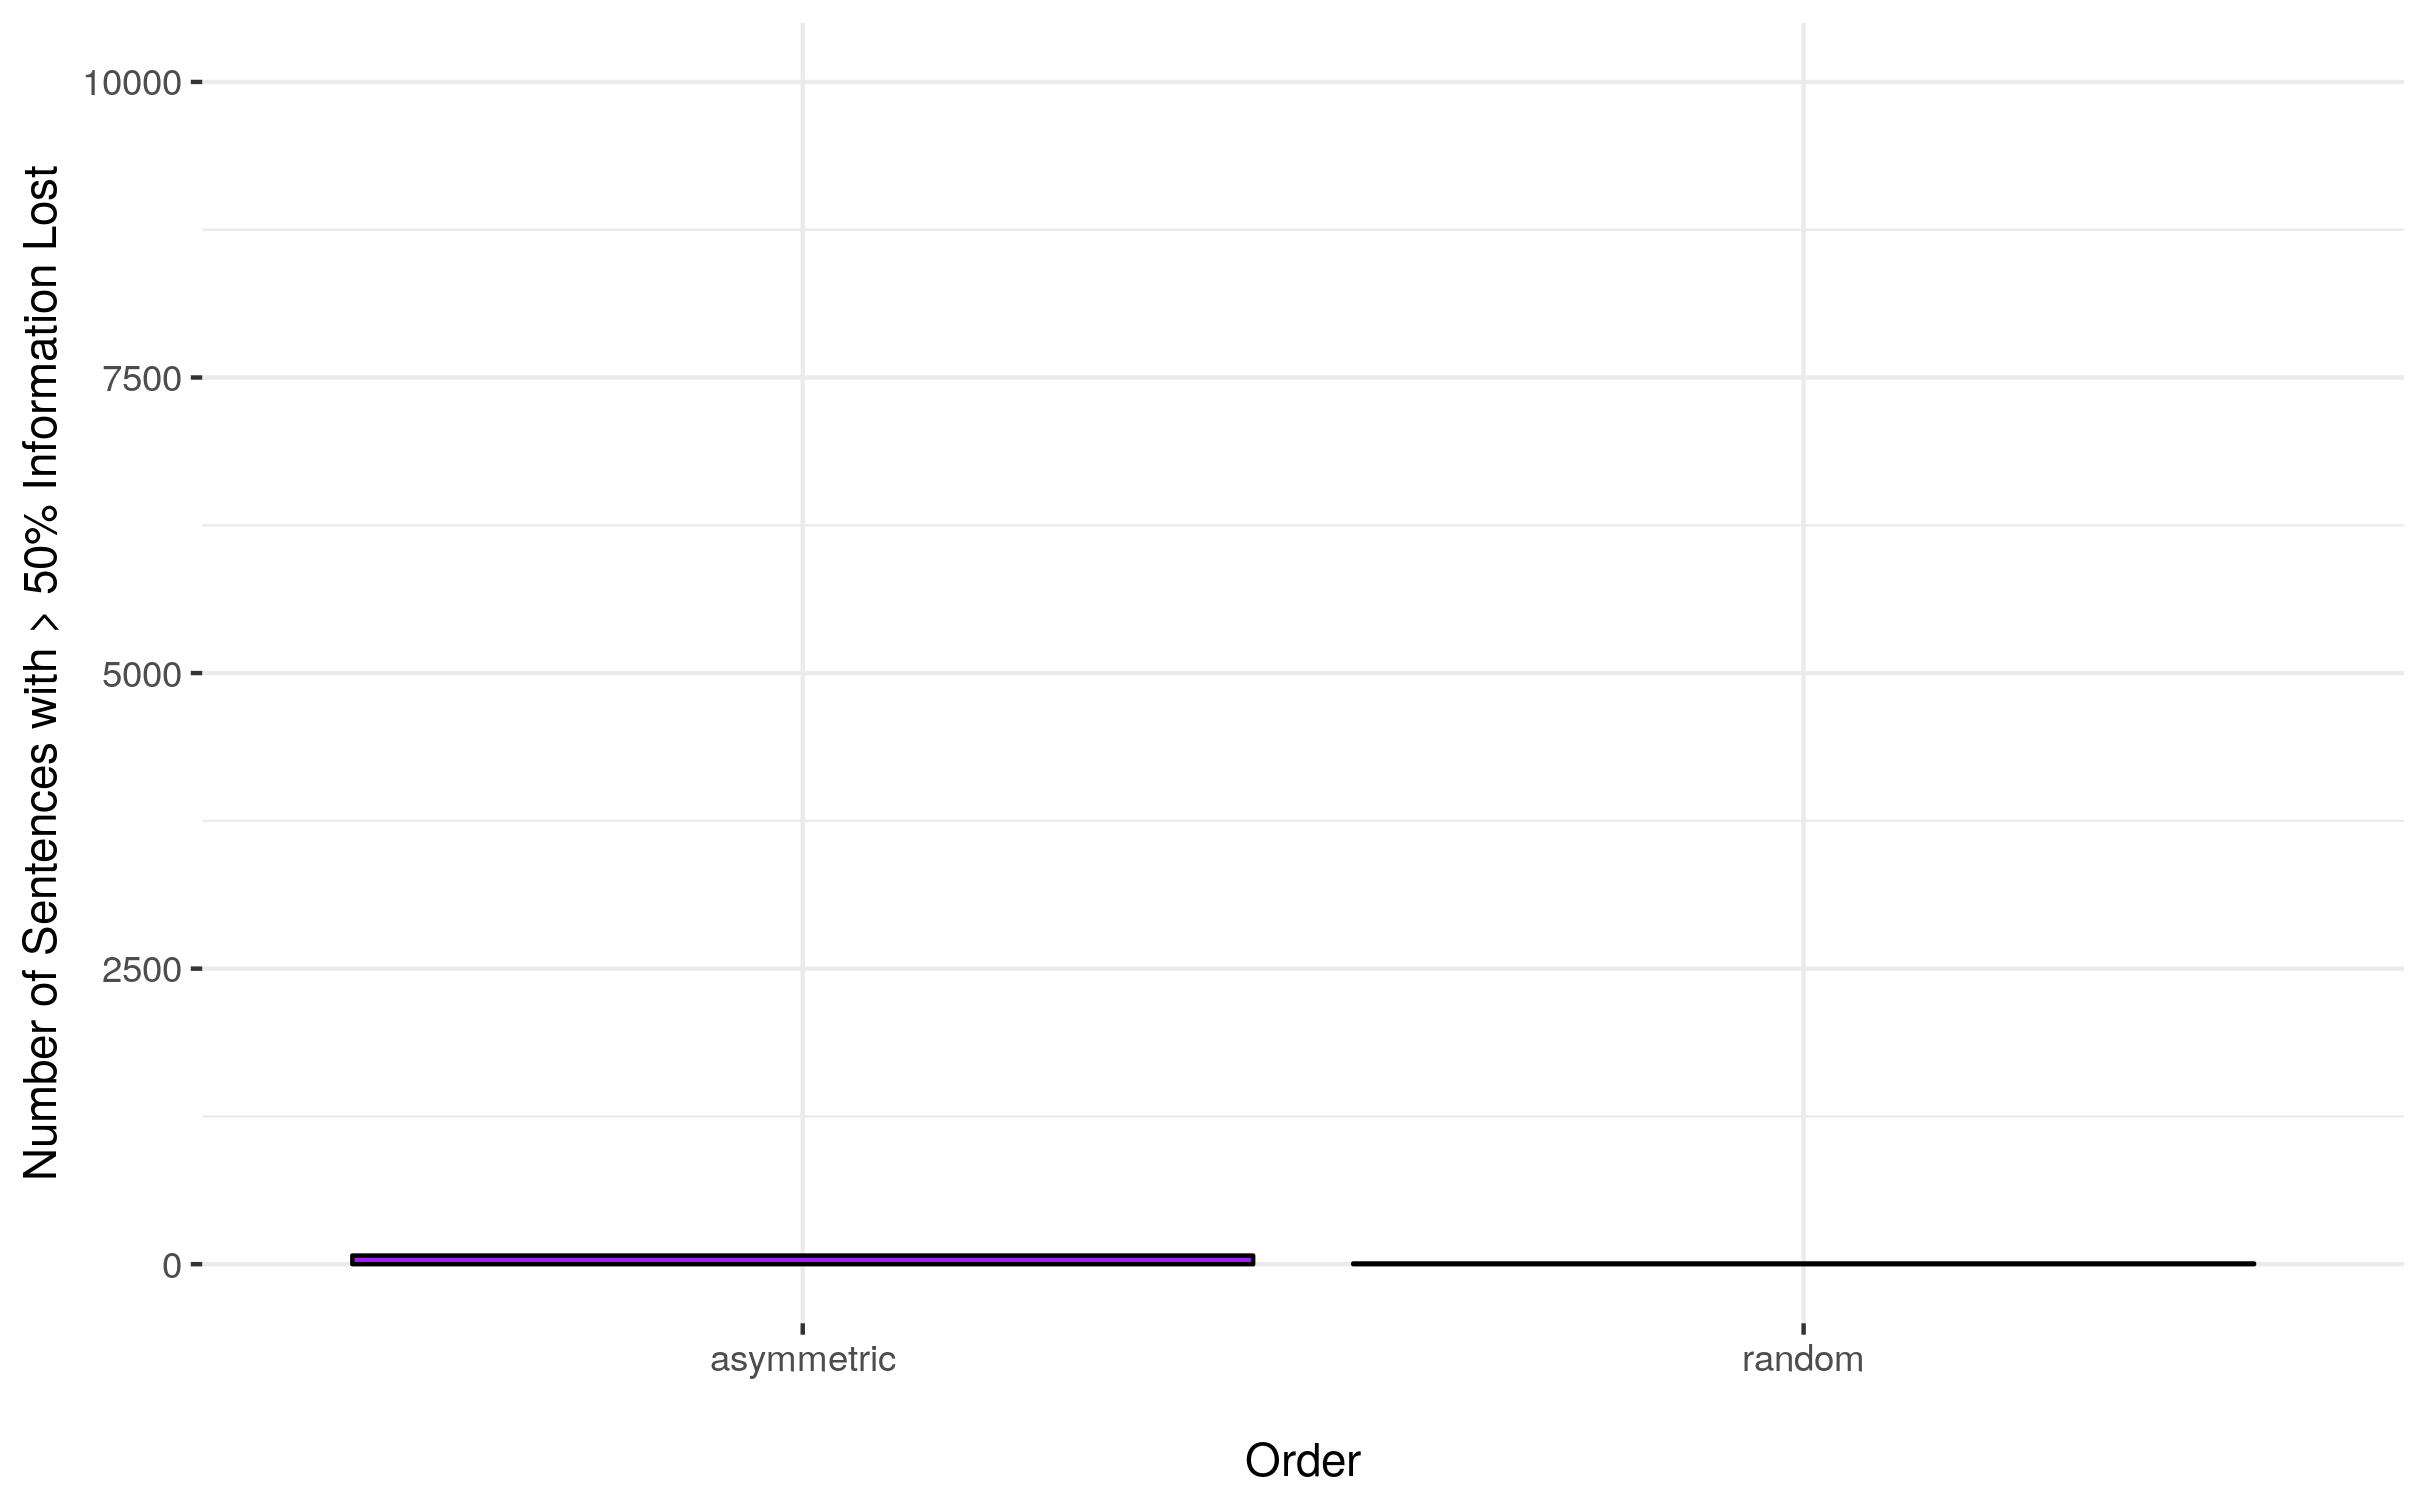
\includegraphics[width=1.115\textwidth]{../uid-sim-majority.png}

\end{frame}

\begin{frame}{Noise Resistance Sim: bits lost and big bit losses} 


\includegraphics[width=1.15\textwidth]{../uid-sim-both.png}

\end{frame}


\section{Language Change}
\subsection{Synctactic change in English}
\begin{frame}
\frametitle{OV to VO Change in English}
\begin{exe} 
	
	\ex \gll tu mihht ec \textbf{gastlike} \textbf{laf} Onn oþerr wise \textyogh arrkenn\\
	you might also spiritual loaf in another way prepare\\
	\quad ``In this way, you will let go of your sins.''\\
	(\textsl{Ormulum}, Lincoln, date: 1200)\\
	\vspace*{5mm}
	\ex \gll Ne {ma\textyogh \textyogh}  he nohht rihht cnawenn \textbf{me}\\
	\sc{neg} may he not right know me\\
	\quad ``He may not rightly know me''\\
	(\textsl{Ormulum}, Lincoln, date: 1200)
	
\end{exe}

\end{frame}

\begin{frame} 
\frametitle{OV to VO Change in English} % \citep{pintzuktaylor2006}
\begin{center}
	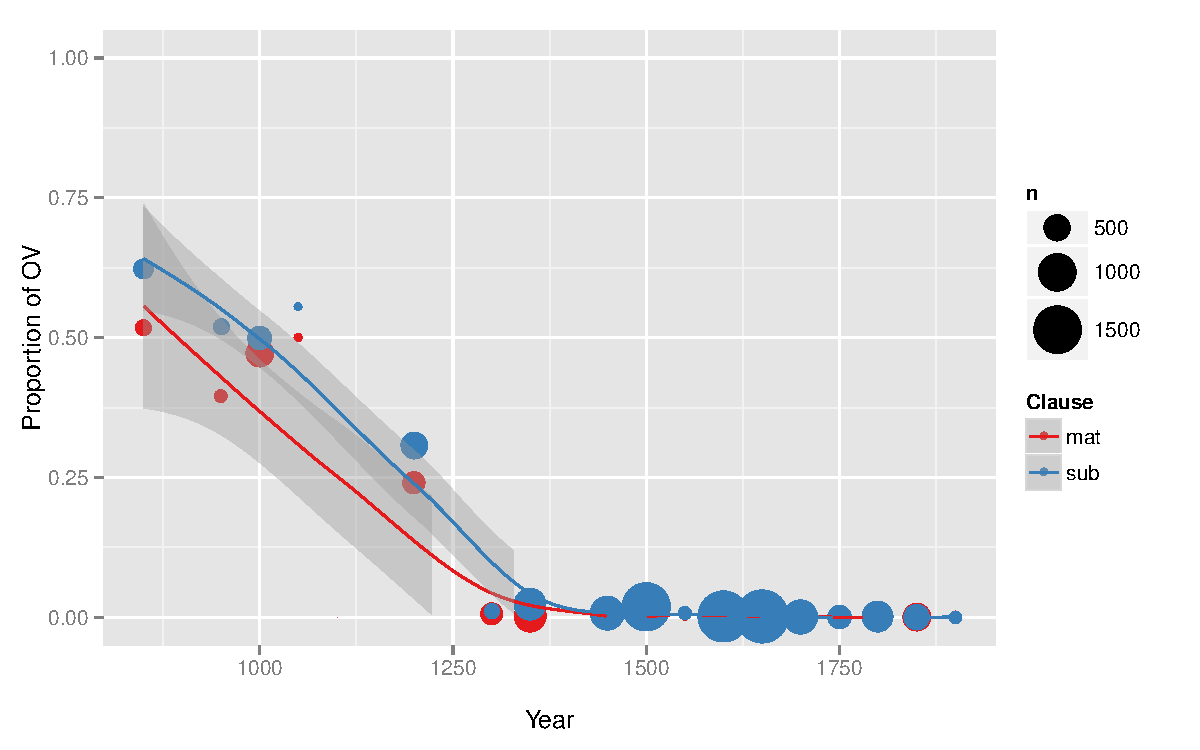
\includegraphics[scale=.6]{myovvoBinnedLoess.pdf}
	%\includegraphics[scale=0.38]{pintzuk.pdf}
\end{center}
\end{frame}

\begin{frame}{Some grammatical preliminaries...}
\begin{exe}
	\ex \textbf{$[$_{Matrix}} Malvina Reynolds implied \textbf{$[$_{Sub}} that you should not like little boxes \textbf{$]$_{Sub} $]$_{Mat}}.
	\ex Malvina Reynolds implied that you should not like them. \textbf{(Pronoun Object)}
	\ex Malvina Reynolds implied that you should not like any/many/most/both/... \textbf{(Quantified Object)}
\end{exe}
\begin{center}
	Guestimated information content hierarchy:\\
	\textbf{Other nominal Obj or Sbj > \\Quantified Obj or Sbj , Verbs > \\Pronoun Obj or Sbj} 
\end{center}
\end{frame}

\begin{frame}{Hypotheses}
\begin{enumerate}
	\item Pronoun subjects should favor OV compared to nominal subjects if the object is nominal: pronSbj-nomObj-V is more uniform in info content than nomObj-nomObj-V, and the latter is less uniform than nomSbj-V-nomObj
	\item Pronoun subjects should do the \textsl{opposite} if the Object is a pronoun: nomSbj-pronObj-V is more uniform than pronSbj-pronObj-V, and the latter is less uniform than pronSbj-V-pronObj.
	\item Quantified Objs should be in-between.
	\item All of these effects should be larger in sub clauses than mat clauses, because of the pressure of preceding information.
\end{enumerate}
\end{frame}


\begin{frame}{OV: Subj and Clause Type, English, N = 28,580} 
%\small{Parsed Corpora: YCOE, PPCME2, PPCEME, PPCMBE}
\nocite{ycoe,ppcme24 ,ppceme,ppcmbe2}

\includegraphics[width=1.115\textwidth]{../infoTheory-posObjsbjmatsub-English.pdf}

\end{frame}



\begin{frame}{OV: Subj, Obj and Clause Type, English} 


 %\small{Parsed Corpora: YCOE, PPCME2, PPCEME, PPCMBE \nocite{ycoe,ppcme2 ,ppceme,ppcmbe}}

\includegraphics[width=1.115\textwidth]{../infoTheory-objsbjmatsub-English.pdf}

\end{frame}

\subsection{Synctactic change in Icelandic}
\begin{frame}{OV: Subj and Clause Type, Icelandic, N = 1,860} 


%\small{Parsed Corpora: YCOE, PPCME2, PPCEME, PPCMBE \nocite{ycoe,ppcme2 ,ppceme,ppcmbe}}

\includegraphics[width=1.115\textwidth]{../infoTheory-posObjsbjmatsub-Ice.pdf}

\end{frame}

\begin{frame}{OV: Subj, Obj and Clause Type, Icelandic}

\nocite{icepahc09}
	%\small{Parsed Corpus: IcePaHC }
	
	\includegraphics[width=1.115\textwidth]{../infoTheory-objsbjmatsubNar-Ice.pdf}
	

\end{frame}






\section{Conclusion}

\begin{frame}{Conclusions}
		\begin{itemize}
			\item Where speakers have an option, i.e. during language change, their choice responds to the resulting density of the entire utterance.
			\item Project with Christine Cuskley and Rachael Bailes to find out whether they also respond to hearer and other factors, and whether we can graduate to actual probabilities in the above work.
			\item MRes student Jack Winter (supervised by Rachael), doing an experiment about rhythm and memory, manipulating information density of symbols in a rhythmic sequence.
			\item ASD vs. typical speakers 
		\end{itemize}
\end{frame}





\begin{frame}{Acknowledgements}
\begin{center}

Thanks to Rachael Bailes, Christine Cuskley, Tony Kroch, among others.
\url{https://github.com/joelcw/constantentropy}\\\vspace{3mm}
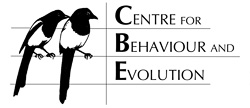
\includegraphics[scale = 0.4]{CBElogo.jpg} 
\end{center}
\end{frame}


\begin{frame}[allowframebreaks]
\frametitle{References}
\newcommand*{\newblock}{natbib}
\bibliographystyle{linquiry2}
\bibliography{joelrefs}
\end{frame}




\end{document}